\documentclass[12pt]{article}
\usepackage[top=1in, bottom=1in, left=1in, right=1in]{geometry}

\usepackage{setspace}
\onehalfspacing

\usepackage{amssymb}
%% The amsthm package provides extended theorem environments
\usepackage{amsthm}
\usepackage{epsfig}
\usepackage{times}
\renewcommand{\ttdefault}{cmtt}
\usepackage{amsmath}
\usepackage{graphicx} % for graphics files
\usepackage{tabu}

% Draw figures yourself
\usepackage{tikz} 

% writing elements
\usepackage{mhchem}

\usepackage{paralist}

% The float package HAS to load before hyperref
\usepackage{float} % for psuedocode formatting
\usepackage{xspace}

% from Denovo Methods Manual
\usepackage{mathrsfs}
\usepackage[mathcal]{euscript}
\usepackage{color}
\usepackage{array}

\usepackage[pdftex]{hyperref}
\usepackage[parfill]{parskip}

% math syntax
\newcommand{\nth}{n\ensuremath{^{\text{th}}} }
\newcommand{\ve}[1]{\ensuremath{\mathbf{#1}}}
\newcommand{\Macro}{\ensuremath{\Sigma}}
\newcommand{\rvec}{\ensuremath{\vec{r}}}
\newcommand{\vecr}{\ensuremath{\vec{r}}}
\newcommand{\omvec}{\ensuremath{\hat{\Omega}}}
\newcommand{\vOmega}{\ensuremath{\hat{\Omega}}}
\newcommand{\even}{\ensuremath{\phi^g}}
\newcommand{\odd}{\ensuremath{\vartheta^g}}
\newcommand{\evenp}{\ensuremath{\phi^{g'}}}
\newcommand{\oddp}{\ensuremath{\vartheta^{g'}}}
\newcommand{\Sn}{\ensuremath{S_N} }
\newcommand{\Ye}[2]{\ensuremath{Y^e_{#1}(\vOmega_#2)}}
\newcommand{\sigg}[1]{\ensuremath{\Macro^{gg'}_{s\,#1}}}
\newcommand{\psig}{\ensuremath{\psi^g}}
%---------------------------------------------------------------------------
%---------------------------------------------------------------------------
\begin{document}
\begin{center}
{\bf NE 255, Fa16 \\
Equation Discretization\\
September 22, 27, and 29, 2016}
\end{center}

\setlength{\unitlength}{1in}
\begin{picture}(6,.1) 
\put(0,0) {\line(1,0){6.25}}         
\end{picture}

Start from the general time-dependent NTE without delayed neutrons, with 7 independent variables. We need to discretize each variable.	
%
\begin{align}
&\frac{1}{v}\frac{\partial \psi}{\partial t}(\rvec,E,\omvec,t) + 
\omvec\cdot  \nabla \psi(\rvec,E,\omvec,t)+
\Sigma_t(\rvec,E)\psi(\rvec,E,\omvec,t)
\\& \quad\quad\quad\quad =
\int_0^{\infty}\int_{4\pi}\Sigma_s(\rvec, E'\rightarrow E,\omvec'\rightarrow\omvec)
\psi(\rvec,E',\omvec',t)d\omvec'dE'\nonumber
\\&\quad\quad\quad\quad\quad\quad +\frac{\chi_p(E)}{4\pi}\int_0^{\infty}\int_{4\pi}\nu(E')\Sigma_f(\rvec,E')
\psi(\rvec,E',\omvec',t)d\omvec'dE'\nonumber
\\&\quad\quad\quad\quad\quad\quad\quad\quad+S(\rvec, E, \omvec,t)\nonumber.
\end{align}

\section*{Time}
Discretize the time interval $[0, T]$ into $N$ timesteps:
%
\begin{figure}[h!]
    \begin{center}
    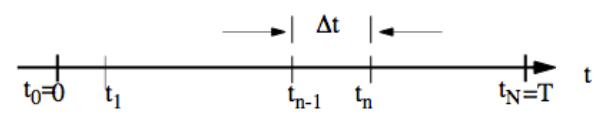
\includegraphics[keepaspectratio, width = 3.5 in]{time}
    \end{center}
\end{figure}
%
Integrate the equation from $t=t_{n-1}$ to $t = t_n$, where we will use the following definitions:
\begin{align*}
\psi(\vec{r}, E ,\vOmega, t_n) &= \psi_n(\vec{r}, E ,\vOmega)\\
\Delta t &= t_{n} - t_{n-1}\\
\bar{\psi}(\vec{r}, E ,\vOmega) &= \frac{1}{\Delta t} \int_{t_{n-1}}^{t_n} dt\: \psi(\vec{r}, E ,\vOmega, t)
\end{align*}
(Note: we're not specifying what actually happens in the integration; we're generically defining a time-averaged angular flux).

We also need to handle the time derivative term so that we can approximate it on a time grid. We will use \textit{First Order Backward Difference} (more on that later): 
\[
\frac{1}{v} \frac{\partial \psi}{\partial t}(\rvec,E,\omvec,t) = \frac{1}{v}\frac{\psi_n(\vec{r}, E ,\vOmega) - \psi_{n-1}(\vec{r}, E ,\vOmega)}{\Delta t}
\]
To get the time behavior of the solution, we integrate the entire transport equation over each time step
\[
\int_{t_{n-1}}^{t_n} dt\: [\cdot]
\]
noting
\[
\int_{t_{n-1}}^{t_n} dt\: \bigl(\frac{1}{v}\frac{\psi_n(\vec{r}, E ,\vOmega) - \psi_{n-1}(\vec{r}, E ,\vOmega)}{\Delta t}\bigr) = \frac{1}{v}\frac{\psi_n(\vec{r}, E ,\vOmega) - \psi_{n-1}(\vec{r}, E ,\vOmega)}{\Delta t}
\]
which gives
\begin{align*}
\frac{1}{v}&\frac{\psi_n(\vec{r}, E ,\vOmega) - \psi_{n-1}(\vec{r}, E ,\vOmega)}{\Delta t} 
+ \omvec\cdot  \nabla  \bar{\psi}(\vec{r}, E ,\vOmega) 
+ \Sigma_t(\rvec,E)\bar{\psi}(\vec{r}, E ,\vOmega) 
= \\& \int_0^{\infty}dE'\int_{4\pi}d\omvec'\: \Sigma_s(\rvec, E'\rightarrow E,\omvec'\rightarrow\omvec) \bar{\psi}(\vec{r}, E' ,\vOmega')
\\&+ \frac{\chi_p(E)}{4\pi}\int_0^{\infty}dE'\:\nu(E')\Sigma_f(\rvec,E')\int_{4\pi}d\omvec'\:
\bar{\psi}(\vec{r}, E' ,\vOmega')
+\bar{S}(\rvec, E, \omvec)
\end{align*}
Note(!): we now have two unknowns ($\psi_n$ and $\bar{\psi}$). We need to relate them; we choose a linear combination with a weighting parameter, $\beta$:
\[
\bar{\psi} = \beta \psi_n + (1 - \beta)\psi_{n-1}
\]
We substitute this in to get
\begin{align*}
\omvec\cdot  \nabla  \bar{\psi}(\vec{r}, E ,\vOmega) 
&+ \bigl(\Sigma_t + \frac{1}{v \beta \Delta t}\bigr)\bar{\psi}(\vec{r}, E ,\vOmega) 
=  \frac{1}{v \beta \Delta t} \psi_{n-1}(\vec{r}, E ,\vOmega) \\
&+ \int_0^{\infty}dE'\int_{4\pi}d\omvec'\: \Sigma_s(\rvec, E'\rightarrow E,\omvec'\rightarrow\omvec) \bar{\psi}(\vec{r}, E' ,\vOmega')
\\&+ \frac{\chi_p(E)}{4\pi}\int_0^{\infty}dE'\:\nu(E')\Sigma_f(\rvec,E')\int_{4\pi}d\omvec'\:
\bar{\psi}(\vec{r}, E' ,\vOmega')
+\bar{S}(\rvec, E, \omvec)
\end{align*}
We solve this for $n=1, \dots, N$ and $\psi_0$ is given (initial value problem!).

%---------------------------------------------------------------------------
\subsubsection*{Aside about Finite Difference}
Finite difference is a common way to numerically approximate derivatives.  \textbf{Example} Given $f$ is $ C^2 \in [a,b]$ and $x_0 \in [a,b]$, find an approximation to $f'(x_0)$ and or $f''(x_0)$, etc.

We're going to come at this from \textbf{Taylor's theorem}, which gives an approximation of a k-times differentiable function around a given point by a k-th order Taylor polynomial.
\[
f(x) = \sum_{0}^{k} \frac{f^{(n)}(x_0)}{n!}(x - x_0)^n
\]
% https://en.wikipedia.org/wiki/Taylor%27s_theorem
To approximate any type of derivative to a specified order of accuracy, we Taylor expand several points in our collection. Then, we choose how many points to combine and in what ways. 
\begin{align*}
f(x_0) &= f(x_0)\\
%
f(x_0 \pm h) &= f(x_0) \pm hf'(x_0) + h^2\frac{f''(x_0)}{2} \pm h^3\frac{f'''(x_0)}{6} + f^{(4)}(c_1)\frac{h^4}{24} \\
%
f(x_0 \pm 2h) &= f(x_0) \pm 2h f'(x_0) + 2 h^2 f''(x_0) \pm \frac{4}{3} h^3 f'''(x_0) + \frac{2}{3}h^4 f^{(4)}(c_2)
\end{align*}
We combine the expanded expressions, rearrange to group terms, and solve for what we want:

For \underline{$O(h)$ Backwards Difference}: combine the point and the next point backward:
\begin{align*}
f(x_0) &= f(x_0)\\
f(x_0 - h) &= f(x_0) - hf'(x_0) + h^2\frac{f''(c)}{2}\\
a f(x_0) &+ b f(x_0 - h) = f'(x_0) \\
a f(x_0) &+ b \bigl(f(x_0) - hf'(x_0) + h^2\frac{f''(c)}{2} \bigr) = f'(x_0) \\
(a+b)f(x_0) &-bh f'(x_0) + b h^2\frac{f''(c)}{2} = f'(x_0)
\end{align*}
%
Now, we solve for the coefficients to get what we want
\begin{align*}
a+b = 0 &\quad -bh = 1 \\
b &= -\frac{1}{h} \quad a = \frac{1}{h}
\end{align*}
%
We now sub in $a$ and $b$. This gives the first order ($O(h)$) Backwards Difference approximation, which is what we used for the time derivative.
\begin{align*}
\text{error }&= -\frac{1}{h}h^2\frac{f''(c)}{2}\\
f'(x_0) &= \frac{f(x_0) - f(x_0 - h)}{h} + \frac{1}{2}hf''(\mu)
\end{align*}

A note about what points to choose: you want to think about how your equations transmit information. 
A perturbation of the initial (or boundary) data of an \textit{elliptic or parabolic} equation is felt at once by essentially all points in the domain.
The solutions of hyperbolic equations are ``wave-like." If a disturbance is made in the initial data of a hyperbolic differential equation, then not every point of space feels the disturbance at once.

%---------------------------------------------------------------------------
%---------------------------------------------------------------------------
\section*{Energy Discretization}
We'd also like to handle the energy dimension by breaking continuous energy into $G$ groups, where group $g$ is [$E_{g}, E_{g-1}$]:
\begin{center}
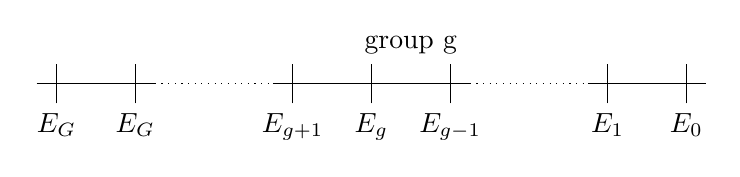
\begin{tikzpicture}
\draw (-.25,0)--(1.25,0);
\draw[dotted] (1.25,0)--(2.75,0);
\draw (2.75,0)--(5.25,0);
\draw[dotted] (5.25,0)--(6.75,0);
\draw (6.75,0)--(8.25,0);
%\draw (4,0)--(5.25,0);
\draw (0,-.25)--(0,.25);
\draw (1,-.25)--(1,.25);
%\draw (2,-.25)--(2,.25);
\draw (3,-.25)--(3,.25);
\draw (4,-.25)--(4,.25);
\draw (5,-.25)--(5,.25);
\draw (7,-.25)--(7,.25);
\draw (8,-.25)--(8,.25);
\node[below] at (0,-.25) {$E_G$};
\node[below] at (1,-.25) {$E_{G}$};
\node[below] at (3,-.25) {$E_{g+1}$};
\node[below] at (4,-.25) {$E_g$};
\node[above] at (4.5, .25) {group g};
\node[below] at (5,-.25) {$E_{g-1}$};
\node[below] at (7,-.25) {$E_{1}$};
\node[below] at (8,-.25) {$E_0$};
\end{tikzpicture}
\end{center}
%
We will solve for group-integrated values in each energy bin using the following definitions:
\begin{align*}
\psi_g(\rvec, \vOmega) &\equiv \int_{E_g}^{E_{g-1}} dE\: \psi(\rvec, \vOmega, E) \qquad
\phi_g(\rvec) \equiv \int_{E_g}^{E_{g-1}} dE\: \phi(\rvec,  E)\\
S_g(\rvec, \vOmega) &\equiv \int_{E_g}^{E_{g-1}} dE\: S(\rvec, \vOmega, E) \qquad
\chi_g \equiv \int_{E_g}^{E_{g-1}} dE\: \chi(E)
\end{align*}
%
To perform these integrals, we need to introduce approximations. We \textit{assume the each item is separable in energy}. For example:
\[
\psi(\vec{r}, \vOmega, E) \approx f(E)\psi_g(\vec{r}, \vOmega)\:, \quad E_g < E \leq E_{g-1}\:,
\]
where $f(E)$ is normalized such that $\int_g dE\: f(E) = 1$.

Next, we need a way to create multigroup cross sections. Options for how to do that in more detail are covered in NE 250. Here we will do the most common/generic approach: weight with the angular flux,
\[\Sigma_{tg}(\vec{r}) \equiv \frac{\int_{E_g}^{E_{g-1}} dE\: \Sigma_t(\rvec, E) f(E)}{\int_{E_g}^{E_{g-1}} dE\: f(E)} = \frac{\int_{E_g}^{E_{g-1}} dE\: \Sigma_t(\rvec, E) \psi(\rvec, \vOmega, E)}{\int_{E_g}^{E_{g-1}} dE\: \psi(\rvec, \vOmega, E)}\]
We do the same thing for fission (not shown here). Scattering requires an extra integral:
\begin{align*}
\Sigma_{s,gg'}(\vOmega' \cdot \vOmega) & \equiv \frac{\int_{E_g}^{E_{g-1}} dE \int_{E_g'}^{E_{g'-1}} dE' \: \Sigma_s(E'\rightarrow E, \vOmega' \cdot \vOmega) f(E')}{\int_{E_g'}^{E_{g'-1}} dE' \: f(E')}\\
& \equiv \frac{\int_{E_g}^{E_{g-1}} dE \int_{E_g'}^{E_{g'-1}} dE' \: \Sigma_s(E'\rightarrow E, \vOmega' \cdot \vOmega) \psi(\rvec, \vOmega', E')}{\int_{E_g'}^{E_{g'-1}} dE' \: \psi(\rvec, \vOmega', E')}
\end{align*}

If we use all of those definitions, we can write a transport equation for each group, $g = 1,\dots, G$:
\begin{align*}
[\vOmega \cdot \nabla + \Sigma_{tg}(\vec{r})]\psi_g(\vec{r}, \vOmega) =&  
\sum_{g'=1}^G \int_{4 \pi} d\vOmega'\: \Sigma_{s,gg'}(\vec{r}, \vOmega' \cdot \vOmega) \psi_{g'}(\vec{r}, \vOmega')\\
&+\frac{\chi_g}{4 \pi}\sum_{g'=1}^G \nu\Sigma_{fg'}(\vec{r}) \phi_{g'}(\vec{r}) + q_g(\vec{r}, \vOmega)
\end{align*}
Giving $G$ coupled equations. Note that the coupling may cause iteration because of the exchange of particles between energy groups (upscattering!). 

These equations are \textbf{exact} in the magical case where (1) the separability in energy holds and (2) the cross sections are constant within each energy group. 


%---------------------------------------------------------------------------
%---------------------------------------------------------------------------
\section*{Angular Discretization}
And the complicated one: angle. We have two main approaches, \textbf{Discrete Ordinates} and \textbf{Spherical Harmonics} (which we often simplify to Legendre polynomials and thus call $P_N$, not to be confused with the scattering expansion).

\subsection*{Discrete Ordinates}
The discrete ordinates approximation is a collocation method in angle. A collocation method is a solution method for ODEs, PDEs, and integral equations. Choose a finite-dimensional space of candidate solutions, such as polynomials up to a certain degree, and a number of points within the domain, called collocation points. Select the solution that satisfies the equation at those points within that space. 
%https://en.wikipedia.org/wiki/Collocation_method

For us, the collocation points are the discrete angles that we choose ($\omvec \rightarrow \omvec_a; a = 1,\dots,n)$ and the solution space is the flux. 
The TE is only valid along the selected set of angles $\vOmega_a$. We apply a compatible quadrature (integration approximation) to the integral term. We write one equation for each angle in the set (dropping energy dependence and fission for simplicity; the source contains scattering and external):
\begin{align*}
\vOmega_a \cdot \nabla \psi_a(\vecr) &+ \Sigma_t(\vecr)\psi_a(\vecr) = Q_a(\vec{r})\\
\psi_a(\vecr) &\equiv \psi(\vecr,\vOmega_a) \qquad Q_a(\vecr) \equiv Q(\vecr,\vOmega_a)\\
\int_{4\pi} d\vOmega\: &= \sum_{a=1}^n w_a = 4\pi \\
\phi(\vecr) &=  \int_{4\pi} d\vOmega\:\psi(\vecr,\vOmega) = \sum_{a=1}^n w_a \psi_a(\vecr)
\end{align*}
The collection ($\vOmega_a, w_a$) is known as the angular quadrature set. The $w_a$ are the integration weights that go with the angles to create an integration. The angle-weight combination + number of angles dictates the accuracy of the integration. The quadrature we choose also dictates the number of unknowns. For Level symmetric, the most common and what people usually mean by $S_{N}$, we get $n=N(N+2)$ unknowns. 

However, we still need to explain what's going on in the sources. To do that, we're going to look at \textit{Spherical Harmonics} and how they relate to Legendre Polynomials. This will allow us to do angular expansions in three dimensions (derived from the Exnihilo manual and Wikipedia). 

\subsubsection*{About Spherical Harmonics}
The addition theorem of Spherical Harmonics can be used to evaluate the
Legendre function, $P_l(\vOmega'\cdot\vOmega)$,
\begin{equation}
  P_l(\vOmega'\cdot\vOmega) = \frac{4\pi}{2l+1}\sum_{m=-l}^l
  Y_{lm}(\vOmega)Y^{\ast}_{lm}(\vOmega')\:,
\end{equation}
where the $Y_{lm}$ are
\begin{equation}
  Y_{lm}(\theta,\varphi) = (-1)^m\sqrt
  {
    \frac{2l+1}{4\pi}\frac{(l-m)!}{(l+m)!}
  }\,
  P_{lm}(\cos\theta)\mathrm{e}^{im\varphi}\:,
  \label{eq:complete-spherical-harmonics}
\end{equation}
and the $P_{lm}$ are the \textit{associated Legendre Polynomials}. These are the solutions to
\[
(1-x^{2}){\frac {d^{2}}{dx^{2}}}P_{\ell }^{m}(x)-2x{\frac {d}{dx}}P_{\ell }^{m}(x)+\left[\ell (\ell +1)-{\frac {m^{2}}{1-x^{2}}}\right]P_{\ell }^{m}(x)=0\:,\]
where the indices $l$ and $m$ are referred to as the degree and order of the associated Legendre polynomial, respectively [before we had called $l$ $n$ and negleced $m$]. When $m$ is zero, these functions are identical to the Legendre polynomials.
%https://en.wikipedia.org/wiki/Associated_Legendre_polynomials

We're going to use Spherical Harmonics to expand our scattering and external source. Everything in our equations must be real; therefore, we can follow a methodology that shows expands a real-valued function using complex Spherical Harmonics ($Y^*$ indicates complex conjugate).  First,
the expansion is split into positive and negative components of $m$,
\begin{equation}
  P_l(\vOmega'\cdot\vOmega) = \frac{4\pi}{2l+1}
  \Bigl[
  Y_{l0}(\vOmega)Y_{l0}(\vOmega') +
  \sum_{m=1}^l
  \bigl(Y_{lm}(\vOmega)Y^{\ast}_{lm}(\vOmega') +
  Y_{l-m}(\vOmega)Y^{\ast}_{l-m}(\vOmega')\bigr)\Bigr]\:.
\end{equation}
Next, we're going to go through a bunch of mathematical maneuvers to get rid of the negative $m$ components and the complex conjugate values. The motivation is ease of analysis and handling. 

First, we'll simplify the $m=0$ term:
\begin{equation}
  Y_{l0} = \sqrt{\frac{2l+1}{4\pi}}\,P_{l0} = Y^e_{l0}\:,
\end{equation}
where we have used the idea that we can separate a spherical harmonic into even and odd components using the $e^{ix}$ identity,
\begin{align}
  Y^e_{lm} &= D_{lm}P_{lm}\cos (m\varphi)\:,\label{eq:Ye}\\
  Y^o_{lm} &= D_{lm}P_{lm}\sin (m\varphi)\:,\label{eq:Yo}\\
  D_{lm} &= (-1)^m\sqrt{(2-\delta_{m0})\frac{2l+1}{4\pi}
    \frac{(l-m)!}{(l+m)!}}\:.
\end{align}

The \(\sqrt{(2-\delta_{m0})\) term appears as an orthogonality requirement. When we expand a function in an entirely \textit{real} basis (as opposed to the complex basis of the general spherical harmonics), the basis functions for the real basis must be orthogonal. The spherical harmonics basis functions are orthogonal, but they also contain complex components that we don't need for real physical quantities such as the scattering source. Hence, the basis functions for the real basis need to be orthogonal, which means that the integral of \(\hat{Y}^e_{lm}\hat{Y}^e_{l'm'}\) over the unit sphere must give unity (with some Kronecker Deltas hanging around as well). We likewise require this orthogonality condition for the odd components. These two orthogonality statements do not give values of 1 unless the definitions contain an extra factor of \(\sqrt{(2-\delta_{m0})\) (the \(\delta_{m0}\) term appears from the orthogonality of cosines in the definition of \(\hat{Y}_{lm}^e\)). 

We will make this substitution in order to satisfy the orthogonality requirement:
\begin{equation}
  \hat{Y}^e_{lm} = \frac{1}{\sqrt{2-\delta_{m0}}}Y^e_{lm}\:,\quad
  \hat{Y}^o_{lm} = \frac{1}{\sqrt{2-\delta_{m0}}}Y^o_{lm}\:.
\end{equation}

Because \(\hat{Y}_{l0}^o=0\) based on the inclusion of \(\sin{(m\phi)}\) in its definition, the above sometimes neglects the \(\delta_{m0}\) term in the odd function since it is implied that \(m=0\) leads to an identically zero function anyways.

Next, we expand the Spherical Harmonics into real and imaginary components. The sum over $m>0$ then becomes 
\begin{equation}
  \sum_{m=1}^l\Bigl(
  \hat{Y}^e_{lm}(\vOmega)\hat{Y}^e_{lm}(\vOmega') +
  \hat{Y}^o_{lm}(\vOmega)\hat{Y}^o_{lm}(\vOmega') +
  \hat{Y}^e_{l-m}(\vOmega)\hat{Y}^e_{l-m}(\vOmega') +
  \hat{Y}^o_{l-m}(\vOmega)\hat{Y}^o_{l-m}(\vOmega')\Bigr)\:,
\end{equation}
where the imaginary terms have been set to zero because our values must be
real. 

Next, we use these relationships to get rid of the $-m$s: 
\begin{align}
 \hat{Y}^e_{l-m} &= (-1)^{-m}\hat{Y}^e_{lm} \equiv (-1)^m\hat{Y}^e_{lm} \:\text{ and}\\
 \hat{Y}^o_{l-m} &= -(-1)^m\hat{Y}^o_{lm}\:,
\end{align}
and then the summation becomes
\begin{equation}
  \sum_{m=1}^l\Bigl(
  2\hat{Y}^e_{lm}(\vOmega)\hat{Y}^e_{lm}(\vOmega') +
  2\hat{Y}^o_{lm}(\vOmega)\hat{Y}^o_{lm}(\vOmega')\Bigr)
\end{equation}
Skipping some steps, we also have the following relationships,

After applying these equations in the $m>0$ terms and combining with the $m=0$
term described above, the expression for $P_l(\vOmega\cdot\vOmega')$ is
\begin{equation}
  P_l(\vOmega'\cdot\vOmega) = \frac{4\pi}{2l+1}
  \Bigl[
  Y^e_{l0}(\vOmega)Y^e_{l0}(\vOmega') +
  \sum_{m=1}^l
  \bigl(Y^e_{lm}(\vOmega)Y^e_{lm}(\vOmega') +
  Y^o_{lm}(\vOmega)Y^o_{lm}(\vOmega')\bigr)\Bigr]\:.
    \label{eq:P_l(mu_o)}
\end{equation}

\subsubsection*{Representing Sources with Spherical Harmonics}
We can use these terms to expand our scattering and external sources (adding energy indexing back in) for multi-D and any degree of anisotropy. The \textbf{scattering source}:

\begin{align}
q^g_{s}(\vec{r},\vOmega) &= \sum_{g'=1}^G \sum_{l=0}^{N} \frac{2l+1}{4 \pi} \Sigma^{gg'}_{sl}(\vecr) \int_{4\pi} d\vOmega'\: P_l(\vOmega \cdot \vOmega') \psi_g(\vecr, \vOmega')\\
  q^g_{s}(\vec{r},\vOmega) &= \sum_{g'=0}^G
  \sum_{l=0}^N
  \sigg{l}(\vec{r})
  \Bigl[
  Y^e_{l0}(\vOmega)\evenp_{l0}(\vec{r}) +
  \sum_{m=1}^l
  \bigl(
  Y^e_{lm}(\vOmega)\evenp_{lm}(\vec{r}) +
  Y^o_{lm}(\vOmega)\oddp_{lm}(\vec{r})
  \bigr)\Bigr]\:,
  \label{eq:mg-scattering-source}
\end{align}
where
\begin{alignat}{3}
  \even_{lm} &= \int_{4\pi}Y^e_{lm}(\vOmega)\psi^g(\vOmega)\:d\vOmega\:,
  \quad& m\ge 0\:,\label{eq:even-flux}\\
  %%
  \odd_{lm} &= \int_{4\pi}Y^o_{lm}(\vOmega)\psi^g(\vOmega)\:d\vOmega\:,
  \quad& m>0\:.\label{eq:odd-flux}
\end{alignat}


Equation~(\ref{eq:mg-scattering-source}) is the multigroup anisotropic
scattering source that is defined by the order of the Legendre expansion,
$P_N$, of the scattering.  For a given $P_N$ order, $(N+1)^2$ moments are
required to integrate the scattering operator.  The moments in
Eqs.~(\ref{eq:even-flux}) and (\ref{eq:odd-flux}) are the \textit{angular flux moments} or, simply, flux moments.
  
Applying the same methodology gives the expansion of the \textbf{external source}
\begin{equation}
  q^g_e(\vec{r}, \vOmega) = \sum_{l=0}^{N}\Bigl[
  Y^e_{l0}(\vOmega)q^g_{l0}(\vec{r}) +
  \sum_{m=1}^{l}
  \bigr(
  Y^e_{lm}(\vOmega)q^g_{lm}(\vec{r}) + Y^o_{lm}(\vOmega)s^g_{lm}(\vec{r})\bigr)
  \Bigr]\:,
  \label{eq:mg-external-source}
\end{equation}
where the spatial dependence has been suppressed.  The even and odd source
moments are defined
\begin{alignat}{3}
  q^g_{lm} &= \int_{4\pi}Y^e_{lm}(\vOmega)q^g_e(\vOmega)\:d\vOmega\:,
  \quad&m\ge 0\:,\label{eq:even-source}\\
  s^g_{lm} &= \int_{4\pi}Y^o_{lm}(\vOmega)q^g_e(\vOmega)\:d\vOmega\:,
  \quad&m>0\:.\label{eq:odd-source}
\end{alignat}

\subsubsection*{Discrete Ordinates Equations}
We put alllll of that together to get
\begin{align*}
\vOmega_a \cdot \nabla \psi^g_a(\vecr) &+ \Sigma^g_t(\vecr)\psi^g_a(\vecr) = \\
&\sum_{g'=0}^G
  \sum_{l=0}^N
  \sigg{l}(\vec{r})
  \Bigl[
  Y^e_{l0}(\vOmega)\evenp_{l0}(\vec{r}) +
  \sum_{m=1}^l
  \bigl(
  Y^e_{lm}(\vOmega)\evenp_{lm}(\vec{r}) +
  Y^o_{lm}(\vOmega)\oddp_{lm}(\vec{r})
  \bigr)\Bigr]\\
&+\sum_{l=0}^{N}\Bigl[
  Y^e_{l0}(\vOmega)q^g_{l0}(\vec{r}) +
  \sum_{m=1}^{l}
  \bigr(
  Y^e_{lm}(\vOmega)q^g_{lm}(\vec{r}) + Y^o_{lm}(\vOmega)s^g_{lm}(\vec{r})\bigr)
  \Bigr]
\end{align*}
The $S_N$ method will be conservative if the quadrature set effectively
integrates the even and odd Spherical Harmonics.

The thing that you solve for is the flux moments, and then you reconstruct that flux at the end.

\subsubsection*{Azimuthal Symmetry}
This all gets simpler if we have azimuthal symmetry. In that case, $m=0$ and 
\[
  Y_{l0}(\theta,\varphi) = (-1)^0\sqrt
  {
    \frac{2l+1}{4\pi}\frac{(l-0)!}{(l+0)!}
  }\,
  P_{l0}(\cos\theta)\mathrm{e}^{i0\varphi} = \sqrt{\frac{2l+1}{4\pi}}P_{l}(\cos\theta),
\]
then 
\begin{align*}
\vOmega_a \cdot \nabla \psi^g_a(\vecr) &+ \Sigma^g_t(\vecr)\psi^g_a(\vecr)  \\
&=\sum_{g'=0}^G
  \sum_{l=0}^N
  \sigg{l}(\vec{r})
  \bigl(
  Y^e_{l}(\vOmega) \evenp_{l}(\vec{r}) \bigr)
+\sum_{l=0}^{N}\bigl(
  Y^e_{l}(\vOmega)q^g_{l}(\vecr)\bigr)\\
  %
 &=\sum_{g'=0}^G
  \sum_{l=0}^N \sigg{l}(\vec{r})\bigl(\sqrt{\frac{2l+1}{4\pi}}P_{l}(\cos\theta)\evenp_{l}(\vec{r}) \bigr)
  + \sum_{l=0}^{N}\bigl(\sqrt{\frac{2l+1}{4\pi}}P_{l}(\cos\theta)q^g_{l}(\vecr)\bigr)
\end{align*}
which is equivalent to what we did in the simplification class.

%-----------------------------------------
\subsubsection*{Discrete Ordinates Considerations}
Two main things to consider in discrete ordinates: \textit{quadrature choice} and \textit{Ray Effects}. 

\textbf{Level Symmetric} quadrature uses the same set of $N/2$ positive values of direction cosines with respect to each of the three axes. That is, for each level $n$ we set $\mu_a = \eta_a = \xi_a$. We describe a level $a$ as the ordinate set that has cosine $\mu_a$ with respect to the $x$ axis. Note that with this setup no axis has preferential treatment. \autoref{fig:levelsym} shows $S_6$. We see there are $6/2 = 3$ values of each direction cosine, and each one is the same wrt each axis. We have $N(N+2)$ quadratures points over the sphere, and that divided by 8 per octant (in this case 48 and 6, respectively). 
\begin{figure}[h!]
    \begin{center}
    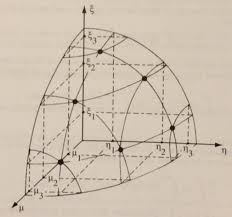
\includegraphics[keepaspectratio, width = 2.5 in]{level-sym}
    \end{center}
    \caption{$S_6$ quadrature}
    \label{fig:levelsym}
\end{figure}

Because of the symmetry constraints not all of the $\mu_n$ are independent. In fact, there is only one degree of freedom because of all of the constraints. Choosing $\mu_1$ sets all of the other values as follows:
\[
\mu_i^2 = \mu_1^2 + \frac{2(1 - 3\mu_1^2)}{N-2}(i-1)\:.
\]
See 4-2 of Lewis and Miller for details. Selecting a $\mu_1$ near the poles will cause clustering at the poles, and so on. 

Further, we need to select weights to perform the integration. These meet the requirement
\[
\sum_{a=1}^{N(N+2)/8} w_a = 1\:.
\]
In the $S_2$ approximation, we only have one choice. For higher values we still have some choices. 

A common choice is to choose weights and angles that correctly integrate as many Legendre Polynomials as possible. These are show in in Table 4-1 in L\&M and are technically called the $LQ_N$ set. There are other $S_N$ versions that have reduced symmetry or relaxation of requirements in other ways. For example, if we don't require all of the cosines to lie on the $N/2$ levels we can maintain rotational symmetry and have equal weights. 

Another common quadrature is \textbf{Gauss-Legendre}. An $n$-point Gaussian quadrature rule is constructed to yield an exact result for polynomials of degree $2n - 1$ or less by a suitable choice of the points $x_i$ and weights $w_i$ for $i = 1, \dots, n$. Common weighting functions include $w(x)= 1/\sqrt{1-x^2}$ (Chebyshev-Gauss) $w(x)=e^{-x^{2}}$ (Gauss-Hermite).
In general, the $n$-th polynomial normalized to give $P_n(1) = 1$, the $i$-th Gauss node, $x_i$, is the $i$-th root of $P_n$; its weight is given by
\[ 
w_{i}={\frac {2}{\left(1-x_{i}^{2}\right)[P'_{n}(x_{i})]^{2}}}.
\]
    %https://en.wikipedia.org/wiki/Gaussian_quadrature
    
    
\textbf{Ray Effects}: ray effects come from the fact that the discrete ordinates method is exact at particular angles, but we cannot say anything about the accuracy at points off of those angles. Consider a point source in a large medium of helium gas. Consider that you've chosen $S_2$. What is the flux going to look like? Consider now that you've chosen $S_14$. What will the flux look like now? It is not very accurate in either case because there is nothing to scatter the neutrons from the angles in question. These are ray effects. 

There are "fix-up" solutions to deal with this. The best approach is probably generating a first collided flux, stopping the calculation, and starting again with the first collision source as the source. This takes the point source, smears it across the space, and allows a diffuse starting source. This functionally improves quite a bit over straight $S_N$ in situations that have unfavorable transport characteristics.

%-----------------------------------------
%-----------------------------------------
\subsection*{Spherical Harmonics, $P_N$ Method}
As mentioned, the other approach is using Spherical Harmonics more broadly. In this method we expand not only scattering and the sources in spherical harmonics, but the flux itself. We're going to go through this in 1-D because that's the most approachable way to do this. Frankly, $P_N$ in multi-D is tough and we don't often do it. When we want multi-D we usually go to simplified $P_N$, which Richard will teach you about next time. 

We will use
\[
\psi(x, \mu) = \sum_{l=0}^{\infty} \frac{(2l+1)}{4\pi} \phi_l(x)P_l(\mu)
\]
for the flux solution in total. This next part comes from Appendix D of L\&M with the normalizations made to be consistent with what we did last class. Note that some people normalize to 1 and some to $4\pi$, which changes the constants. I'll try to be consistent... We start with the within group, 1D TE
\[
\mu \frac{\partial \psi}{\partial x} + \Sigma_t(x)\psi(x,\mu) = \sum_{l=0}^{\infty} \frac{(2l+1)}{4\pi} \Sigma_{s,l}(x) P_l(\mu)\phi_l(x) + S(x,\mu)
\]
where $S(x,\mu)$ is the group source given by
\[
S(x,\mu) = \sum_{l=0}^{\infty} \frac{(2l+1)}{4\pi} P_l(\mu) \sum_{g' \neq g} \Sigma_{sl,gg'}(x) \phi_{lg'}(x) + \tilde{S}_g(x,\mu)
\]
with $\tilde{S}_g(x,\mu)$ being the external and/or fission source for the group. 
(This is breaking the group summation into the within group component and the scattering across other groups component).\\
Recall: as long as the series is infinite, we are not introducing any approximations.

------------------------------------\\
A note on translating between $P_l(\mu_0)$, where $\mu_0 - \vOmega \cdot \vOmega'$, and $P_l(\vOmega')P_l(\vOmega)$:
\begin{align*}
\Sigma_s(\vOmega' \cdot \vOmega) &= \sum_{l=0}^{\infty} \frac{2l+1}{4\pi} \Sigma_{sl} P_l(\mu_0) = \sum_{l=0}^{\infty} \frac{2l+1}{4\pi} \Sigma_{sl} P_l(\vOmega')P_l(\vOmega) \\
%\psi(x, \mu) &\approx \sum_{l=0}^{\infty} \frac{(2l+1)}{4\pi} \phi_l(x)P_l(\mu)\\
\phi_l(x) &= \int d\mu \: P_{l}(\mu)\psi(x,\mu)\\
%
&\sum_{l=0}^{\infty} \frac{2l+1}{4\pi} \Sigma_{sl}(x) \int_{-1}^1 d\mu'\: P_l(\mu_0) \psi(x, \mu') =  \sum_{l=0}^{\infty} \frac{2l+1}{4\pi} \Sigma_{sl}(x) \int_{-1}^1 d\mu'\: P_l(\mu)P_{l}(\mu')\psi(x,\mu') \\
%
&\sum_{l=0}^{\infty} \frac{(2l+1)}{4\pi} \Sigma_{s,l}(x) P_l(\mu)\phi_l(x)  = \sum_{l=0}^{\infty} \frac{(2l+1)}{4\pi} \Sigma_{s,l}(x)\int d\mu' \: P_l(\mu)P_{l}  (\mu')\psi(x,\mu')
\end{align*}
------------------------------------

We can use the Legendre expansion to make our TE an infinite set of coupled ODEs. We use the flux expansion in the equation, multiply by $P_{l'}(\mu)$ and integrate over $-1 \leq \mu \leq 1$:
\begin{align*}
\sum_{l=0}^{\infty} &\frac{(2l+1)}{4\pi}\biggl[\int_{-1}^1 d\mu\: \mu P_{l'}(\mu) P_l(\mu) \frac{d}{d x}\phi_l(x) +  \int_{-1}^1 d\mu\: P_{l'}(\mu) P_l(\mu) \Sigma_t(x)\phi_l(x) \biggr] \\
&= \sum_{l=0}^{\infty} \frac{(2l+1)}{4\pi} \Sigma_{sl}\int_{-1}^1 d\mu\: P_{l'}(\mu) P_l(\mu) \phi_l(x) + s_{l'}(x)
\end{align*}
where
\[
s_{l'}(x) = \int_{-1}^1 d\mu\:P_{l'}(\mu) s(x,\mu)\:.
\]
We use the orthogonality relation
\[
\int_{-1}^1 d\mu\: P_{l'}(\mu) P_l(\mu) = \frac{2\delta_{l l'}}{2l+1}
\]
to remove the summation in the collision and scattering terms. \\
However, the streaming term requires more work. We will use the Legendre recursive relationship
\[
\mu P_l(\mu) = \bigl(\frac{l+1}{2l+1}\bigr)P_{l+1}(\mu) + \bigl(\frac{l}{2l+1}\bigr)P_{l-1}(\mu)
\]
to get rid of $\mu$. This all gives, for $l' = 0, 1, \dots$
\[
\bigl(\frac{l'+1}{2l'+1}\bigr)\frac{d}{d x}\phi_{l'+1}(x) + \bigl(\frac{l'}{2l'+1}\bigr)\frac{d}{d x}\phi_{l'-1}(x) + \Sigma_t(x) \phi_{l'} = \Sigma_{sl'}(x)\phi_{l'}(x) + s_{l'}(x)\:.
\]
what do we do when $l'=0$ for $\phi_{-1}$? We typically just set it to $0$, which doesn't matter anyway since we don't technically use that moment, giving
\[
\frac{d}{dx}\phi_1(x) + (\underbrace{\Sigma_t - \Sigma_{s0}}_{\Sigma_a})\phi_0(x) = s_0(x)
\]
This is one equation with two unknowns. Let's try $l=1$:
\[
\frac{2}{3}\frac{d}{dx}\phi_2(x) + \frac{1}{3}\frac{d}{dx}\phi_0(x) + (\Sigma_t - \Sigma_{s1})\phi_1(x) = s_1(x)
\]
Every time we add another equation we get another unknown, so we now have a closure problem.\\
To deal with this, we make the $P_N$ \textit{approximation}. We set either 
\[\phi_{N+1} = 0 \quad\text{ or }\quad\frac{d}{dx}\phi_{N+1}=0
\]
(which gives the same effect) to get $N+1$ coupled equations. 

We can see that diffusion theory is the $P_1$ approximation.\\
If we have an isotropic source, $s_1=0$. Use this in the $l=1$ equation to see
\[
\phi_1(x) = \frac{-1}{3(\Sigma_t - \Sigma_{s1})}\frac{d \phi_0}{dx}
\]
where $\phi_1$ is also known as the net current--so we've got Fick's Law.\\
The $l=0$ equation is then
\[
\frac{-1}{3(\Sigma_t - \Sigma_{s1})}\frac{d^2 \phi_0}{dx^2} + \Sigma_a \phi_0(x) = s_0(x)\:.
\]

In practice, we only ever select $N$ to be odd. This allows us to use $(N+1)/2$ conditions for each of the left and right boundaries. \\
This is much easier than having odd boundary conditions would end up introducing artificial asymmetry. \\
Using $N$ = even doesn't provide more information either. Look at $N=2$ (recall $\phi_3 = 0$):
\begin{align*}
\frac{2}{5}&\frac{d}{dx}\phi_1(x) +(\Sigma_t - \Sigma_{s2})\phi_2(x) = s_2(x)\\
&\\
\phi_2(x) &= \frac{s_2(x) - \frac{2}{5}(\overbrace{s_0(x) - \Sigma_a(x)\phi_0(x)}^{\text{from }l=0})}{\Sigma_t - \Sigma_{s2}}
\end{align*}
$\phi_0$ and $\phi_2$ are linearly dependent, which is not thought to give you better accuracy.\\
When we use $N$ = odd, we don't have this dependence in our last equation. 


We also need to actually set these \textbf{boundary conditions}.
\begin{itemize}
\item \underline{Interface}: $\psi(x,\mu)$ is continuous across every interface. Since
\[
\phi_l = \int_{-1}^1 d\mu\: \mu P_{l}(\mu)\psi(x,\mu)
\]
this condition implies that each $\phi_l(x)$ must also be continuous across that interface. 

\item \underline{Reflective} (extendable to periodic): for some reflecting surface $x_s$:
\begin{align*}
\psi(x_s,\mu) &= \psi(x_s,-\mu) \quad \mu \in [0,1]\\
\sum_{l=0}^{\infty} \frac{(2l+1)}{4\pi}\phi_l(x_s)P_l(\mu) &= \sum_{l=0}^{\infty} \frac{(2l+1)}{4\pi}\phi_l(x_s)\underbrace{P_l(-\mu)}_{(-1)^l P_l(\mu)}\\
\sum_{l=0}^{\infty} \frac{(2l+1)}{4\pi}\phi_l(x_s)P_l(\mu)\bigl[1 - (-1)^l\bigr] &= \sum_{l=1}^{\infty} \frac{(2l+1)}{4\pi}\phi_l(x_s)\underbrace{P_l(-\mu)}_{(-1)^l P_l(\mu)}\\
&= 0 \quad \text{for odd }l
\end{align*}
Because $P_l(\mu)$ are mutually independent, 
\[\boxed{\phi_l(x_s) =0\text{ for odd }l}\]

\item \underline{Vacuum}: These are trickier in this approximation. If there are no neutrons entering from the right at a boundary $x_0$, the exact condition would be
\[
\psi(x_0, \mu) = 0\:, \quad -1 \leq \mu < 0\:.
\]
However, when we truncate the Legendre expansion we can't meet this exactly (because it implies a discontinuity in the flux at $\mu=0$).\\
Instead, we need other conditions. There are two choices.\\
(1) \textit{Mark BCs}: we set
\[
\psi(x_0, \mu_n) = 0\:, \quad n = 1, 2, \dots, \frac{N+1}{2}
\]
where 
\[
P_{N+1}(\mu_n) = 0\:.
\]
This is the analytical solution of our coupled equations in a source-free, pure absorber from $x_0 \leq x \leq \infty$.

(2) \textit{Marshak BCs}: we simply set the odd angular moments to zero. 
\[
\int_{-1}^0 d\mu\: P_{l}(\mu)\psi(x_0,\mu) = 0\:, \quad n = 1, 3, 5, \dots, N
\]
This condition sets the net number of neutrons entering the solid identically to zero, which we can see from $l=1$:
\[
\int_{-1}^1 d\mu\: \mu \psi(x_0,\mu) = 0\:.
\]
This is the same as saying $J^-(x_0) = 0$ and thus this boundary condition holds even when only using $P_1$. \\
We usually choose the Marshak as it generally introduces less error.  
\end{itemize}

There are some major \textit{deficiencies} of $P_N$. \\
We get poor representation of $\psi$ near vacuum boundaries. We can use Double $P_N$ ($DP_N$) to deal with this (which we're not going to cover in this class).\\


\subsection*{Approximation Errors}
With discrete ordinates, errors can be removed through spatial integration. The physical oscillations in the flux will balance out, and the magnitudes are pretty correct. Further, you can visually see ray effects--so you can tell that something is going on. You can increase the order, and you can see what might or might not be trustworthy. 

With $P_N$ the errors are often in magnitude rather than shape, so it is much more difficult to assess whether your solution is correct. (in complex geometries it is also sometimes hard to tell for ray effects). 


\end{document}
